\chapter{Global Statistics}
\label{chap:global_statistics}

MPAS-Ocean simulations create global statistics text files that are accessible during the simulation, as described in Table \ref{oceanTable:global statistics}.  These are useful to check the health and progress of a simulation, and to compare the history of global statistics amongst similar simulations.  Frequency is controlled by \verb|_stats_| flags in the namelist.  The files are simply text files formatted in columns and rows, where each row is a particular time, written to \verb|stats_time.txt|, and each column is a variable, described in \verb|stats_readme.txt|.  Output is always appended to the {\tt stats\_*} files, so these files must be deleted or moved in order to restart from line one.

A chain of simple unix commands may be used to access a specific part of the data.  For example, to view the last three values of column seven in the global average, use
\begin{verbatim}
cat stats_avg.txt | awk '{print $7}' | tail -n3
\end{verbatim}
Gnuplot is a simple plotting tool available on Linux systems that can easily plot columns in text files.  In this example, two MPAS-Ocean simulations were executed, in directories \verb|run1| and \verb|run2|.  Begin Gnuplot with the \verb|gnuplot| command at the unix prompt.  Plot column seven from both runs using points with
\begin{verbatim}
plot 'run1/stats_avg.txt' u 7 w p, 'run2/stats_avg.txt' u 7 w p
\end{verbatim}
and with lines using
\begin{verbatim}
plot 'run1/stats_avg.txt' u 7 w l, 'run2/stats_avg.txt' u 7 w l
\end{verbatim}
Plot on a vertical log scale and add legend text with
\begin{verbatim}
set logscale y
plot 'run1/stats_avg.txt' u 7 w l t 'run 1', 'run2/stats_avg.txt' u 7 w l t 'run 2'
\end{verbatim}
It is often useful to view the difference between the global statistics of two simulations.  This can be done with the paste command, which concatenates the two files horizontally.  In this example, each file has 18 columns, so \$25 refers to column 7 of the second file:
\begin{verbatim}
plot '<paste run1/stats_avg.txt run2/stats_avg.txt' u ($7-$25)
\end{verbatim}

\begin{table}[ht] 
\caption{Global statistics output files.}
\vspace{0.5cm} \centering 
\begin{tabular}{ll} 
\hline\hline file name & description  \\
\hline 
\verb|stats_time.txt| & time stamp, rows correspond to rows of other stats files \\
\verb|stats_readme.txt| & list of variables in columns of other stats files \\
\verb|stats_min.txt| & minimum over the global domain \\
\verb|stats_max.txt| & maximum over the global domain \\
\verb|stats_sum.txt| & volume-weighted summation over the global domain \\
\verb|stats_avg.txt| & volume-weighted average over the global domain \\
\verb|stats_colmin.txt| & minimum column sum over the global domain \\
\verb|stats_colmax.txt| & maximum column sum over the global domain \\
\hline 
\end{tabular} \label{oceanTable:global statistics} 
\end{table}

\begin{figure}[H!]
	\centering
	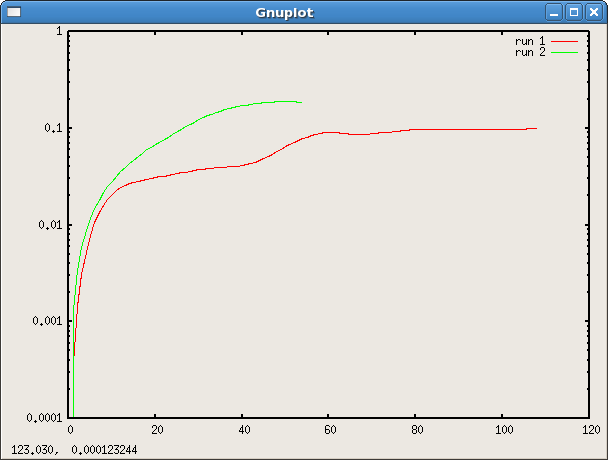
\includegraphics[scale=0.5]{ocean/figures/gnuplot.png}
	\caption{Example of plot of global statistics created with gnuplot.}
	\label{fig:gnuplot}
\end{figure}
